\documentclass[deutsch]{llncs}

\usepackage{url}
\usepackage{graphicx}
\usepackage{listings}
\usepackage{verbatim}
\usepackage{listings}
\lstset{numberbychapter=false}
\usepackage[lined,linesnumbered,german]{algorithm2e}
\SetAlCapFnt{\small}
\SetAlCapNameFnt{\small}
\usepackage{tikz}
\usetikzlibrary{arrows,automata}
\usepackage{xspace}

% for german seminar theses
\usepackage[utf8]{inputenc}
\usepackage[ngerman]{babel}
\usepackage{csquotes}
\usepackage[abbreviate=false,maxbibnames=99,backend=bibtex]{biblatex}
\bibliography{referenzen}

\usepackage{hyperref}

\setcounter{secnumdepth}{2}
\setcounter{tocdepth}{3}

% define custom macros for specific formats or names
\newcommand{\uml}[1]{\texttt{#1}\xspace}
\newcommand{\cd}{\textsf{Klassendiagramm}\xspace}

% Numeriere 3 Ebenen tief (bis subsection)
\setcounter{secnumdepth}{2}

% make a proper TOC despite llncs
\setcounter{tocdepth}{2}
\makeatletter
\renewcommand*\l@author[2]{}
\renewcommand*\l@title[2]{}
\makeatletter

\begin{document}
\def\abstractname{Kurzfassung.}

\pagestyle{plain}
\pagenumbering{roman}

\title{Virtuelle und erweiterte Realtität\thanks{Diese Arbeit wurde im Rahmen der LVA ``Wissenschaftliches Arbeiten'' (188.925) im WS18 erstellt.}}


%&&&&&&&&&&&&&&&&&&&&&&&&&&&&&&&&&&&&&&&&&&&&&&&&&&&&&&&&&&&&&&&&&&&&&&&&
% Name and address of the author
%&&&&&&&&&&&&&&&&&&&&&&&&&&&&&&&&&&&&&&&&&&&&&&&&&&&&&&&&&&&&&&&&&&&&&&&&
%\author{Max Mustermann}

%\institute{Technische Universität Wien\\ Bachelorstudium Wirtschaftsinformatik\\ \email{max.mustermann@tuwien.ac.at} \\ Matrikelnr.: 0123456}

%&&&&&&&&&&&&&&&&&&&&&&&&&&&&&&&&&&&&&&&&&&&&&&&&&&&&&&&&&&&&&&&&&&&&&&&&
% Example for more than one authors
%&&&&&&&&&&&&&&&&&&&&&&&&&&&&&&&&&&&&&&&&&&&&&&&&&&&&&&&&&&&&&&&&&&&&&&&&
\author{Barbara Elias\inst{1} \and Wang Yi\inst{2}}

\institute{Technische Universität Wien\\ Bachelorstudium Wirtschaftsinformatik\\ \email{e1028094@student.tuwien.ac.at} \\ Matrikelnr.: 1028094
\and
Technische Universität Wien\\ Bachelorstudium Technische Informatik\\ \email{martina.musterfrau@student.tuwien.ac.at} \\ Matrikelnr.: 0234567}

\maketitle

% reset footnote counter in case of multiple authors
\setcounter{footnote}{0}

\begin{abstract}
Die Kurzfassung fasst den Inhalt Ihrer Seminararbeit mit 70 bis 150 Wörtern zusammen. \dots
\end{abstract}

%&&&&&&&&&&&&&&&&&&&&&&&&&&&&&&&&&&&&&&&&&&&&&&&&&&&&&&&&&&&&&&&&&&&&&&&&
% Table of contents
% Activate or deactivate this according to the guideline instructor
%&&&&&&&&&&&&&&&&&&&&&&&&&&&&&&&&&&&&&&&&&&&&&&&&&&&&&&&&&&&&&&&&&&&&&&&&
\tableofcontents
\newpage

\pagenumbering{arabic}

\section{Einleitung}
\label{sec:intro}
Dieses Dokument dient als Vorlage und Leitfaden und soll Autoren beim Erstellen ihrer Seminararbeit unterstützen. Die Beurteilung richtet sich nach der Qualität der theoretischen und/oder praktischen Arbeit sowie nach der Struktur, Inhalt und Formulierung der schriftlichen Seminararbeit. Berücksichtigen Sie insbesondere die Grundlagen wissenschaftlichen Arbeitens (zB korrekte Zitierung).

\section{Gestaltung der Kapitel}
\label{sec:typo}

Für das Arbeiten mit LaTeX können Sie auf eine Vielzahl von Bücher sowie auf im Internet frei verfügbare Einführungen und Tutorials zurückgreifen. Eine gute erste Anlaufstelle für LaTeX  Beginner ist das LaTeX  Wikibook, verfügbar unter \url{http://en.wikibooks.org/wiki/LaTeX}.

Im Folgenden werden die wichtigsten LaTeX-Umgebungen und Befehle beispielhaft beschrieben.

\subsection{Tabellen}
\label{subsec:tables}

Tabellarische Darstellungen sind mit Hilfe der Tabellen-Umgebung zu erstellen. Tabellen werden fortlaufend nummeriert und mit einem kurzen Titel versehen (siehe Tabelle \ref{tab:diplomandenseminar}).

\begin{table}[htb]
	\caption{DiplomandInnenseminar}
	\label{tab:diplomandenseminar}
    \centering	
	\begin{tabular}{|l|c|c|}
		\hline \textbf{Name} & \textbf{Termin} & \textbf{Thema} \\
		\hline
		\hline Mustermann Max  & 18.5   & T1    \\
		\hline Musterfrau Martina  & 22.6   & T2    \\
		\hline
	\end{tabular}
\end{table}


\subsection{Abbildungen}
\label{subsec:fig}

Wie Tabellen sind auch Abbildungen fortlaufend zu nummerieren und mit einer kurzen Bildunterschrift zu versehen. Sie können Grafiken direkt in LaTeX mit Hilfe von PSTricks\footnote{\url{http://tug.org/PSTricks}}, Tikz\footnote{\url{http://sourceforge.net/projects/pgf}}, oder einer beliebigen Bibliothek gestalten, die Ihre Anforderungen erfüllt (siehe Abbildung~\ref{fig:samplefigure_tikz}). Alternativ können Grafiken in externen Bildbearbeitungsprogrammen gestaltet werden und in dieses Dokument eingebunden werden (siehe Abbildung~\ref{fig:samplefigure}). Beachten Sie dabei, dass alle Abbildungen eine Auflösung von mindestens 300 dpi aufweisen um eine hohe Druckqualität zu erzielen.

\begin{figure}
	\centering
	\begin{tikzpicture}[->, auto, node distance=2.8cm, semithick]
	  \node[initial, state] (1)		 {$S_1$};
	  \node[state] 		(2) [right of=1] {$S_2$};
	
	  \path (1) edge [bend left]  node {0} (2)
		(1) edge [loop above] node {1} (1)
		(2) edge [bend left]  node {0} (1)
		(2) edge [loop above] node {1} (2);
	\end{tikzpicture}
	\caption{Beispielabbildung TIKZ}
	\label{fig:samplefigure_tikz}
\end{figure}

\begin{figure}[tb]
	\centering
	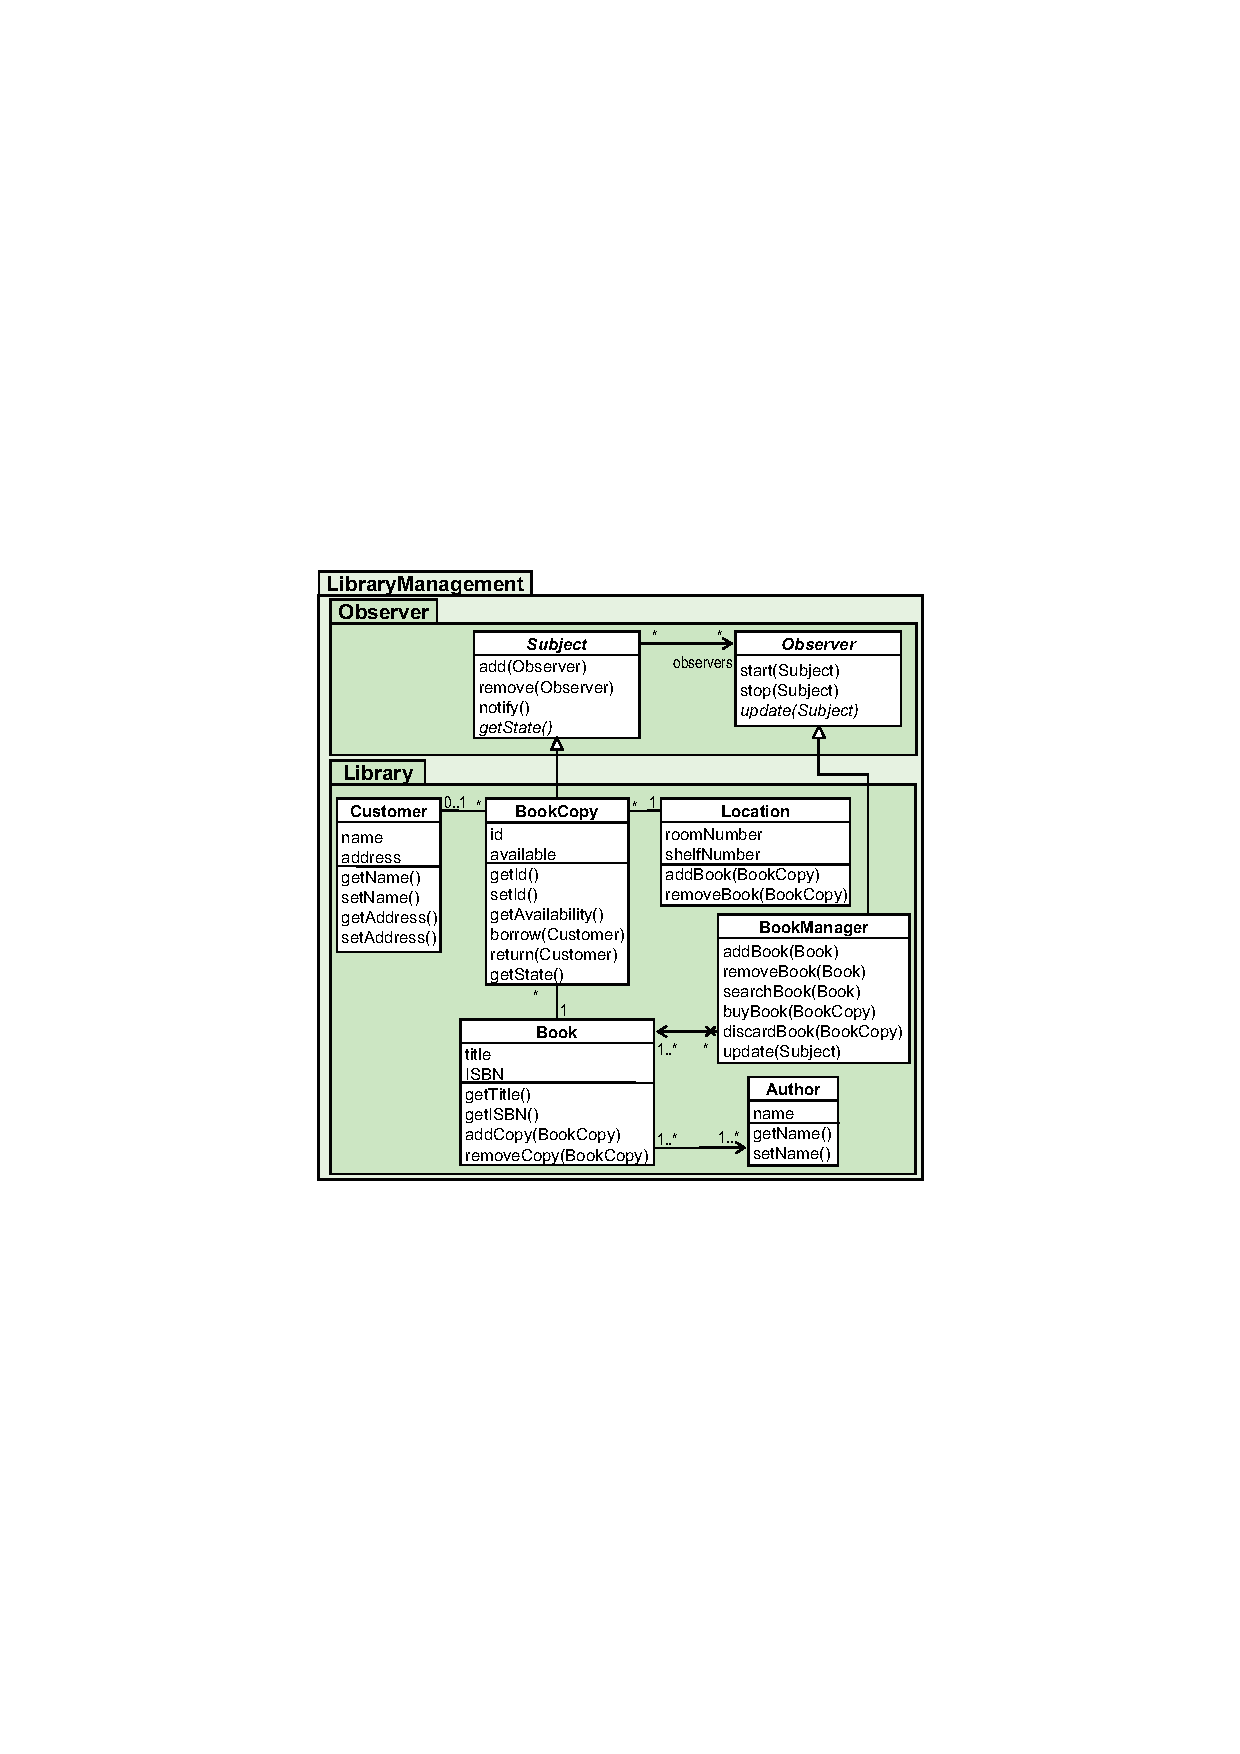
\includegraphics[width=0.7\textwidth]{figures/figure1}
	\caption{Beispielabbildung PDF}
	\label{fig:samplefigure}
\end{figure}


\subsection{Schriftarten}
\label{subsec:fonts}

Wenn Sie wichtige Begriffe zum ersten mal einsetzen, verwenden Sie eine \emph{kursive} Schriftart. 
Um ein konsistentes Schriftbild zu gewährleisten, können Sie für wiederkehrende Namen wie \cd oder \uml{Observer} Muster im Hauptdokument \texttt{seminararbeit.tex} Makros definieren. 

\subsection{Code}
\label{subsec:code}

Für kurze Programmausschnitte benutzen Sie die Verbatim-Umgebung.

\begin{verbatim}
//Start Program
System.out.println("Hello World!");
//End Program
\end{verbatim}

Eine sehr viel bessere Möglichkeit bieten die Algorithmen-Umgebung bzw. die Listings-Umgebung (siehe Algorithmus~\ref{alg:samplealgorithm} und Listing~\ref{lst:hello}). Diese Umgebungen bieten besondere Formatierungsfunktionen für Schlüsselwörter, Schleifen, Operationen und Kommentare. 

\begin{algorithm}[t]
\SetKwData{Left}{left}
\SetKwData{This}{this}
\SetKwData{Up}{up}
\SetKwFunction{Union}{Union}
\SetKwFunction{FindCompress}{FindCompress}
\SetKwInOut{Input}{input}
\SetKwInOut{Output}{output}

\Input{A bitmap $Im$ of size $w\times l$}
\Output{A partition of the bitmap}

\BlankLine

\emph{special treatment of the first line}\;
\For{$i\leftarrow 2$ \KwTo $l$}{
\emph{special treatment of the first element of line $i$}\;
\For{$j\leftarrow 2$ \KwTo $w$}{\label{forins}
\Left$\leftarrow$ \FindCompress{$Im[i,j-1]$}\;
\Up$\leftarrow$ \FindCompress{$Im[i-1,]$}\;
\This$\leftarrow$ \FindCompress{$Im[i,j]$}\;
\If(\tcp*[r]{O(\Left,\This)==1}){\Left compatible with \This}{\label{lt}
\lIf{\Left $<$ \This}{\Union{\Left,\This}}\;
\lElse{\Union{\This,\Left}\;}
}
\If(\tcp*[r]{O(\Up,\This)==1}){\Up compatible with \This}{\label{ut}
\lIf{\Up $<$ \This}{\Union{\Up,\This}}\;
\tcp{\This is put under \Up to keep tree as flat as possible}\label{cmt}
\lElse{\Union{\This,\Up}}\tcp*[r]{\This linked to \Up}\label{lelse}
}
}
\lForEach{element $e$ of the line $i$}{\FindCompress{p}}
}
\caption{Beispielalgorithmus}\label{alg:samplealgorithm}
\end{algorithm}

% use minipage environment around listings to circumvent page breaks
\begin{minipage}{\linewidth} 
\lstset{%
  basicstyle=\sffamily,
  keywordstyle=\bfseries,
  columns=fixed,
  showstringspaces=false,
  language=Java
}  
\begin{lstlisting}[caption={Hello world}, label=lst:hello, captionpos=b]
//Start Program
if (true) {
    System.out.println("Hello World!");
}
//End Program
\end{lstlisting}
\end{minipage}

\section{Literaturverweise}
\label{sec:bib}

\subsection{Literatursuche}
\label{subsec:search}

Informationen zu Online-Bibliotheken sowie zur Literatursuche, d.h. interessante Zeitschriften, Konferenzen und Organisationen, finden Sie unter \url{http://www.big.tuwien.ac.at/teaching/info.html}.

\subsection{BibTeX}
\label{subsec:bibtex}
Verwenden Sie für die einzelnen Literaturverweise BibTeX.

Im LaTeX Quelldokument dieses pdf Dokuments finden Sie verschiedene Beispiele für Referenzen auf Journals~\cite{jour:B2BServices}, Konferenzartikel~\cite{proc:TheWebMLApproach}, Bücher~\cite{book:umlatwork}, Buchkapitel~\cite{incoll:ErhardKonrad1992}, elektronische Standards~\cite{man:BPEL}, Dissertationen~\cite{phdthesis:manuelWimmer}, Masterarbeiten~\cite{mast:AUMLProfile} und Webseiten~\cite{misc:BIGWebsite}. Die zugehörigen BibTeX Einträge finden Sie in der Datei \texttt{referenzen.bib}. Für die Verwaltung der BibTeX Referenzen können Sie zB \url{http://www.citeulike.org} bzw. JabRef für die Offline-Verwaltung verwenden.

\printbibliography

\end{document}
